 %% Stefan Nagel Dissertation
%%%%%%%%%%%%%%%%%%%%%%%%%%%%%%%%%%%%%%%%%%%%%%%%%%%%%%%%%%%%%

%%%%%%%%%%%%%%%%%%%%%%%%%%%%%%%%%%%%%%%%%%%%%%%%%%%%%%%%%%%%%
%% HEADER
%%%%%%%%%%%%%%%%%%%%%%%%%%%%%%%%%%%%%%%%%%%%%%%%%%%%%%%%%%%%%
\documentclass[
paper=A5,
fontsize = 10pt, % 10pt for a5
DIV=14, % division of text to frame --> scrguide
BCOR=8mm, % bindenkorrektur
twoside,
open=any, % open chapter on any page
parskip = half,
toc = index,
toc = bibliography,
draft = false, %instead of final
pagesize=pdftex, % scrguide s.52 einstellung des papierformats
numbers=noenddot,
version=last
]{scrbook}




%% Language %%%%%%%%%%%%%%%%%%%%%%%%%%%%%%%%%%%%%%%%%%%%%%%%%
% pakete
\usepackage[USenglish]{babel} % find typos
%\usepackage[ansinew]{inputenc} % sourceencoding
%\usepackage{mathpazo} % palatino, s. l2tabu
%\usepackage[scaled=.95]{helvet}
%\usepackage{Times}
%\usepackage[T1]{fontspec}
%\setmainfont{Times}
\usepackage{microtype} % stretches some words to get rid of some over/underfull boxes
%\usepackage{mathptmx} % times 
%\usepackage[scaled=.95]{helvet}
\usepackage{times}

%\usepackage[pdftex, final]{graphicx} % figures for pdfLaTeX
%\usepackage{subfigure}

\usepackage{amsmath} % amsmath
\usepackage{amssymb} % amsmath symbols
\usepackage{stackrel} % math own operators
%\usepackage{nicefrac} % makes nice view of 1/2 or 1/4 especially in text

\usepackage{float}
%\usepackage{listings} % sourcecode listings
%\lstloadlanguages{C, Python}
%\lstset{numbers=left, numberstyle=\tiny, numbersep=5pt, basicstyle=\ttfamily, breaklines=true}
%\lstset{language=C}
%\usepackage{multicol}

\usepackage{booktabs}
\usepackage{multirow} % for cells over multiple rows in tables
%\usepackage{tabularx}
\usepackage{longtable}
%\usepackage{acronym}
%\usepackage[acronym]{glossaries} % acronyms, glossary and notations 

\usepackage{makeidx}
\usepackage{lscape} % for figures in landscape --> chapter 3 --> USRP signal flow
\usepackage{rotating} % for figures in landscape --> chapter 3 --> USRP signal flow
%\usepackage{sistyle}
\usepackage{textcomp}

%% Use url and break them if they are too long for the page
\usepackage[hyphens]{url}

% Removes the highliting around the hyperlinks 
%\usepackage[pdfborder={0 0 0},bookmarksopen]{hyperref}
\usepackage{hyperref}
\usepackage[hyphenbreaks]{breakurl}

\usepackage{scrhack} %removes warning by redefinition of macros float@addtolist etc
\usepackage{todonotes}


\usepackage[framemethod=TikZ]{mdframed} %% For inserting the individual contributions in box
\mdfdefinestyle{MyFrame}{%
    linecolor=blue,
    outerlinewidth=0.8pt,
    roundcorner=8pt,
    %innertopmargin=\baselineskip,
    %innerbottommargin=\baselineskip,
    %innerrightmargin=20pt,
    %innerleftmargin=20pt,
%    backgroundcolor=gray!50!white
}

\hypersetup{ % properties of pdf
  pdftitle={Performance Analysis of Cognitive Radio Systems with Imperfect Channel Knowledge},
  pdfauthor={M.Sc. Ankit Kaushik},
  pdfsubject={Dissertation},
  pdfcreator={LaTeX},
  pdfproducer={LaTeX und Co.},
  pdfkeywords={Cognitive Radio, Performance Analysis, Imperfect Channel Knowledge}
 }
\usepackage{import}	% To provide relative paths
\usepackage[caption=false,font=footnotesize]{subfig} %% Plotting Subfigures
\usepackage{color,psfrag}  % Because most of matlab figures are generated with laprint that generates a .tex(with psfrag commands) and .eps


\usepackage{tikz}   % Drawing tool that overlaps on the plotted figures
\usepackage{siunitx} %SI notations looks nice
\usepackage[retainorgcmds]{IEEEtrantools}
%\renewcommand{\IEEEProof}[Solution]
\renewcommand{\IEEEQED}{}

%\usepackage[numbers]{natbib}
\usepackage[resetlabels, labeled]{multibib}	%% Generate document with multiple bibliography
\newcites{K}{Related Publications} 
\usepackage{cite} % Combining multiple citations
%\include{cite}

\hyphenation{centra-lity knowl-edge throu-ghput fra-mework domi-nant esti-mation-throughput}

%\usepackage{rotating} % Rotate the text sideways
%\usepackage{adjustbox}% Rotate the text sideways

\makeindex

%% Redefine Spacing for the table of contents 
%\usepackage[subfigure]{tocloft}
%\renewcommand\cftchapafterpnum{\vskip4pt}
%\renewcommand\cftsecafterpnum{\vskip4pt}
%\renewcommand\cftsubsecafterpnum{\vskip4pt}
%\setlength{\cftsubsecnumwidth}{10em}

\usepackage{etoolbox}

%\makeatletter
%\pretocmd{\chapter}{\addtocontents{toc}{\protect\addvspace{15\p@}}}{}{}
%\pretocmd{\section}{\addtocontents{toc}{\protect\addvspace{15\p@}}}{}{}
%\makeatother
%% Modifying chapter style
\usepackage{titlesec}
\titleformat{\chapter}[display]
  {\huge}
  {\filcenter\MakeUppercase{\chaptertitlename} \huge\thechapter}
  {1ex}
  {\titlerule[1pt]\vspace{1ex}\filcenter}
  [\vspace{1ex}{\titlerule[1pt]}]


%\graphicspath{{./../kapitel05/}}
%% Important macros and notations used in the dissertation are defined here

\newif\ifdebug
\debugfalse


\makeatletter
\if@twocolumn
	\newcommand{\figscalet}{0.71 \columnwidth}
	\newcommand{\figscalett}{\columnwidth}
	\newcommand{\figscale}{0.77 \columnwidth}
\else
	\newcommand{\figscale}{0.73\columnwidth}
	\newcommand{\figscalet}{0.7 \columnwidth}
	\newcommand{\figscalett}{\columnwidth}
\fi
\makeatother

% General Commands  
\newcommand{\e}[2]{{\mathbb E}_{#1}\left[ #2 \right]}    % Expectation
\newcommand{\s}[2]{{\frac{1}{{#1}}\sum_{n=1}^{#1}} {#2}}     % Summation 
\newcommand{\q}[2]{{\mathcal Q}_{#1}\left( #2 \right)}   % Macum Q function 
\newcommand{\p}{\mathbb P}				 % Probability
\newcommand{\sub}[1]{_{\text{#1}}}		         % Subscript as text
\newcommand{\supe}[1]{^{\text{#1}}}


% Probability 
\newcommand{\pd}{\text{P}\sub{d}}			 % Detection Probability 
\newcommand{\pfa}{\text{P}\sub{fa}}			 % False alarm Probability 
\newcommand{\pco}{\text{P}\sub{c}}			 % Confidence Probability 
\newcommand{\phz}{\p(\mathcal{H}_0)}                     % 0 Hypothesis  
\newcommand{\pho}{\p(\mathcal{H}_1)}			 % 1 Hypothesis  

%% Discrete Signals
\newcommand{\yrcvd}{y\sub{ST}}
\newcommand{\xp}{x\sub{PT}}
\newcommand{\xsfull}{x\sub{ST}}
\newcommand{\xscont}{x\sub{ST,cont}}
\newcommand{\ps}{P\sub{s}}
\newcommand{\ys}{y\sub{SR}}
\newcommand{\nap}{w}
\newcommand{\nas}{w}
\newcommand{\yp}{y\sub{PR}}
\newcommand{\xreg}{x\sub{ST,cont}}
\newcommand{\xtran}{x\sub{PR}}
\newcommand{\xtranpr}{x\sub{PR}}
\newcommand{\xtranst}{x\sub{ST}}
\newcommand{\xs}{x\sub{ST}}




% Signal to noise ratio
\newcommand{\snrp}{\frac{\ptranpt}{\npo}}
\newcommand{\snrs}{\frac{\ptranst}{\npo}}
\newcommand{\snrsi}{\frac{\npo}{\ptranst}}
\newcommand{\snrst}{\frac{\ps}{\sigma^2}}
\newcommand{\snrrcvd}{{\gamma}\sub{p,1}}
\newcommand{\snrso}{{\gamma}\sub{s}}
\newcommand{\snrpt}{{\gamma}\sub{p,2}}
\newcommand{\snrfull}{{\gamma}\sub{s, full}}
\newcommand{\snrcont}{{\gamma}\sub{s, cont}}
\newcommand{\snrsp}{\frac{|\ehs|^2 \ptranst}{\npo}\Big /\frac{\eprcvdsr}{\npo}}


% Distribution parameters 
\newcommand{\ls}{\lambda\sub{s}}
\newcommand{\Ks}{N\sub{s}}
\newcommand{\lp}{\lambda\sub{p}}
\newcommand{\Kp}{N\sub{p,2}}
\newcommand{\lpo}{\lambda\sub{p,1}}
\newcommand{\lpt}{\lambda\sub{p,2}}

\newcommand{\apo}{a\sub{p,1}}
\newcommand{\bpo}{b\sub{p,1}}
\newcommand{\apt}{a\sub{p,2}}
\newcommand{\bpt}{b\sub{p,2}}
\newcommand{\as}{a\sub{s}}
\newcommand{\bs}{b\sub{s}}
\newcommand{\ap}{a\sub{2}}
\newcommand{\bp}{b\sub{2}}

\newcommand{\mpo}{m\sub{p,1}}
\newcommand{\mpt}{m\sub{p,2}}
\newcommand{\ms}{m\sub{s}}
\newcommand{\acc}{\beta}


% Channel gain and power gain 
\newcommand{\hpo}{h\sub{p,1}}
\newcommand{\hptw}{h\sub{p,2}}
\newcommand{\hpth}{h\sub{p,3}}
\newcommand{\hs}{h\sub{s}}
\newcommand{\hpt}{h\sub{p,2}}

% Power
\newcommand{\ptran}{P\sub{Tx,PR}}
\newcommand{\preg}{P\sub{Tx,ST,cont}}
\newcommand{\pfull}{P\sub{Tx,ST,full}}
\newcommand{\npp}{\sigma^2\sub{w}}
\newcommand{\nps}{\sigma^2\sub{w}}
\newcommand{\npu}{\Delta\sigma^2}
\newcommand{\npo}{\sigma^2\sub{w}}
\newcommand{\spo}{\sigma^2\sub{s}}
\newcommand{\prcvdstpt}{P\sub{Rx,ST,$\hpo$}}
\newcommand{\prcvdsr}{P\sub{Rx,SR}}
\newcommand{\prcvdstpr}{P\sub{Rx,ST,$\hpth$}}
\newcommand{\ptranst}{P\sub{Tx,ST}}
\newcommand{\ptranpt}{P\sub{Tx,PT}}
\newcommand{\ptranpr}{P\sub{Tx,PR}}
\newcommand{\prcvdpr}{P\sub{Rx,PR}}
\newcommand{\prcvd}{P\sub{Rx,ST}}
\newcommand{\pp}{P\sub{p}}
\newcommand{\evar}{\frac{\npo}{2 \Ks}}


% Estimated parameters 
\newcommand{\eprcvdstpt}{\hat{P}\sub{Rx,ST,$\hpo$}}
\newcommand{\eprcvdstpr}{\hat{P}\sub{Rx,ST,$\hpth$}}
\newcommand{\eprcvdsr}{\hat{P}\sub{Rx,SR}}
\newcommand{\eprcvdpr}{\hat{P}\sub{Rx,PR}}
\newcommand{\epreg}{\hat{P}\sub{Tx,ST,cont}}
\newcommand{\ephs}{|\hat{h}\sub{s}|^2}
\newcommand{\ehpo}{\hat{h}\sub{p,1}}
\newcommand{\egpo}{\hat{h}\sub{p,1}}
\newcommand{\egpt}{\hat{h}\sub{p,2}}
\newcommand{\epgpo}{|\hat{h}\sub{p,1}|^2}
\newcommand{\epgpt}{|\hat{h}\sub{p,2}|^2}
\newcommand{\epgs}{|\hat{h}\sub{s}|^2}
\newcommand{\ehs}{\hat{h}\sub{s}}
\newcommand{\eprcvd}{\hat{P}\sub{Rx,ST}}
\newcommand{\ecz}{\hat{\text{C}}\sub{0}}
\newcommand{\eco}{\hat{\text{C}}\sub{1}}
\newcommand{\ectw}{\hat{\text{C}}\sub{2}}
\newcommand{\ecth}{\hat{\text{C}}\sub{3}}
\newcommand{\epd}{\hat{\text{P}}\sub{d}}
\newcommand{\eca}{\hat{\text{{C}}}\sub{s}}
\newcommand{\ers}{\hat{\text{{R}}}\sub{s}}
\newcommand{\ephpth}{|h\sub{p,3}|^2}

% Channels parameters
\newcommand{\phpo}{|h\sub{p,1}|^2}
\newcommand{\phptw}{|h\sub{p,2}|^2}
\newcommand{\phpth}{|h\sub{p,3}|^2}
\newcommand{\phs}{|h\sub{s}|^2}
\newcommand{\gpo}{h\sub{p,1}}
\newcommand{\gpt}{h\sub{p,2}}
\newcommand{\gs}{h\sub{s}}
\newcommand{\pgpo}{|h\sub{p,1}|^2}
\newcommand{\pgpt}{|h\sub{p,2}|^2}
\newcommand{\egs}{\hat{h}\sub{s}}
\newcommand{\pgs}{|h\sub{s}|^2}
\newcommand{\phpt}{|h\sub{p,2}|^2}


% System and performance paramters
\newcommand{\fsam}{f\sub{s}}
\newcommand{\flo}{f\sub{LOOfsset}}
\newcommand{\tsen}{\tau\sub{sen}}
\newcommand{\testpt}{\tau\sub{est, $\hpo$}}
\newcommand{\testptsr}{\tau\sub{est, $\hptw$}}
\newcommand{\testpr}{\tau\sub{est, $\hpth$}}
\newcommand{\ttestpt}{\tilde{\tau}\sub{est, $\hpo$}}
\newcommand{\ttestptsr}{\tilde{\tau}\sub{est, $\hptw$}}
\newcommand{\ttestpr}{\tilde{\tau}\sub{est, $\hpth$}}
\newcommand{\ttest}{\tilde{\tau}\sub{est}}
\newcommand{\ttsen}{\tilde{\tau}\sub{sen}}
\newcommand{\rs}{R\sub{s}}
\newcommand{\rsz}{R\sub{0}}
\newcommand{\rso}{R\sub{1}}
\newcommand{\rstw}{R\sub{2}}
\newcommand{\rsth}{R\sub{3}}
\newcommand{\trs}{R\sub{s}}
%\newcommand{\ers}{\e{}{\rs}}

\newcommand{\ca}{\text{C}\sub{s}}
\newcommand{\ttau}{\tilde{\tau}}

\newcommand{\test}{\tau\sub{est}}
\newcommand{\ttesto}{{\tau}^*\sub{est}}
\newcommand{\ttsenac}{\tilde{\tau}\sub{sen}\supe{}}
\newcommand{\ttsenoc}{\tilde{\tau}\sub{sen}\supe{}}

\newcommand{\rsac}{R\sub{s}\supe{AC}}
\newcommand{\rsoc}{R\sub{s}\supe{OC}}
\newcommand{\trsac}{{R}\sub{s}\supe{}}
\newcommand{\trsoc}{{R}\sub{s}\supe{}}


\newcommand{\cz}{\text{C}\sub{0}}
\newcommand{\co}{\text{C}\sub{1}}
\newcommand{\ctw}{\text{C}\sub{2}}
\newcommand{\cth}{\text{C}\sub{3}}

% Constraints and Thresholds
\newcommand{\ite}{\theta\sub{I}}     				% Interference Threshold
\newcommand{\opc}{\rho\sub{cont}}                               % Outage Probability Constraint on Controlled Power   
\newcommand{\opdc}{\rho\sub{d}}
\newcommand{\pdd}{\bar{\text{P}}\sub{d}}
\newcommand{\pcod}{\bar{\text{P}}\sub{c}}			 % Constraint on Confidence Probability 
\newcommand{\pc}{P\sub{Tx,ST,full}}
\newcommand{\mpd}{\rho\sub{d}}
\newcommand{\thric}{\mu\sub{IC}}
\newcommand{\thrac}{\mu\supe{}}
\newcommand{\throc}{\mu\supe{}}



% Distribution functions
\newcommand{\feprcvdstpt}{F_{\eprcvdstpt}}			% Estimated received power for the link ST - PT
\newcommand{\feprcvdstpr}{F_{\eprcvdstpr}}                      % Estimated received power for the link ST - PR 
\newcommand{\feprcvdsr}{F_{\eprcvdsr}}                          % Estimated received power for the link PT - SR 
\newcommand{\fprcvdpr}{F_{\eprcvdpr}}
\newcommand{\fephs}{F_{\ephs}}                                  % Estimated received power for the link ST - SR 
\newcommand{\fpd}{F_{\epd}}
\newcommand{\fcz}{F_{\ecz}}
\newcommand{\fco}{F_{\eco}}
\newcommand{\fctw}{F_{\ectw}}
\newcommand{\fcth}{F_{\ecth}}
\newcommand{\fprcvd}{F_{\eprcvd}}
\newcommand{\fgs}{F_{\epgs}}
\newcommand{\fgp}{F_{\epgpo}}
\newcommand{\fc}{F_{\ca}}
\newcommand{\fprcvdsr}{F_{\eprcvdsr}}
\newcommand{\fpreg}{F_{\epreg}}
\newcommand{\fpgpo}{F_{\pgpo}}
\newcommand{\fpgpt}{F_{\pgpt}}
\newcommand{\fpgs}{F_{\pgs}}
\newcommand{\feprcvd}{F_{\eprcvd}}
\newcommand{\fphpo}{F_{\phpo}}
\newcommand{\fphpt}{F_{\phpt}}
\newcommand{\fphs}{F_{\phs}}

% Density functions
\newcommand{\dprcvdstpt}{f_{\prcvdstpt}}
\newcommand{\dpreg}{f_{\epreg}}
\newcommand{\dhs}{f_{\hs}}
\newcommand{\drs}{f_{\ers}}
\newcommand{\dcz}{f_{\ecz}}
\newcommand{\dco}{f_{\eco}}
\newcommand{\dctw}{f_{\ectw}}
\newcommand{\dcth}{f_{\ecth}}
\newcommand{\dpd}{f_{\epd}}
\newcommand{\dc}{f_{\ca}}
\newcommand{\dsnrs}{f_{\frac{ |\ehs|^2 \ptranst}{\npo}}}
\newcommand{\dsnrp}{f_{\frac{\eprcvdsr}{\npo}}}
\newcommand{\dsnrsp}{f_{\frac{|\ehs|^2 \ptranst}{\npo}\Big /\frac{\eprcvdsr}{\npo}}}
\newcommand{\dprcvd}{f_{\eprcvd}}
\newcommand{\dprcvdpr}{f_{\eprcvdpr}}


\newcommand{\imp}{\uline}
\newcommand{\ur}{\uuline}
\newcommand{\ns}{\uwave} 
\newcommand{\ws}{\sout}
\newcommand{\fl}{\dashuline}
\newcommand{\un}{\dotuline}

% Define new mathmatical operators 
\DeclareMathOperator*{\maxi}{max}
\DeclareMathOperator*{\gthan}{\ge}
\DeclareMathOperator*{\eqto}{=}
\DeclareMathOperator*{\cchi2}{\mathcal{X}^2}
\DeclareMathOperator*{\ncchi2}{\mathcal{X}_1^2}
\DeclareMathOperator*{\ts}{\text{T}(\textbf{y})}
\DeclareMathOperator*{\argmaxi}{argmax}


% Theorem Stuff
\newtheorem{theorem}{Theorem}
\newtheorem{case}{Case}
\newtheorem{constraint}{Constraint}
\newtheorem{lemma}{Lemma}
\newtheorem{prop}{Proposition}
\newtheorem{remark}{Remark}
\newtheorem{coro}{Corollary}
\newtheorem{defi}{Definition}
\newtheorem{approxi}{Approximation}

% derrived Expressions
\newcommand{\lambdas}{\frac{\sigma_w^4}{ 2 \Ks \ptranst}}
\newcommand{\lambdasinv}{\frac{2 \Ks \ptranst}{\sigma_w^4}}




% Used to break the theorems, proof between the columns
\allowdisplaybreaks


%%%%%%%%%%%%%%%%%%%%%%%%%%%%%%%%%%%%%%%%%%%%%%%%%%%%%%%%%%%%%
%% DOCUMENT
%%%%%%%%%%%%%%%%%%%%%%%%%%%%%%%%%%%%%%%%%%%%%%%%%%%%%%%%%%%%%
\begin{document}




\frontmatter

%% Title Page %%%%%%%%%%%%%%%%%%%%%%%%%%%%%%%%%%%%%%%%%%%%%%%

%% The simple version:
%\title{Portable Waveform Development for Software Defined Radios}
%\author{Dipl.-Ing. Stefan Nagel}
%\date{} %%If commented, the current date is used.
%\maketitle

%% The final version

% Leeres Blatt einfuegen f�r Widmung
%\newpage
%\thispagestyle{empty}
%\section*{}
%\cleardoublepage


% Titelseite aus Grafik

%% Uncomment this to make the following appear
%\thispagestyle{empty}

%\todo{Cover Image}
%\begin{figure}[]
%\vspace{-1.5cm}
%\hspace{-1.9cm}
%\centering
%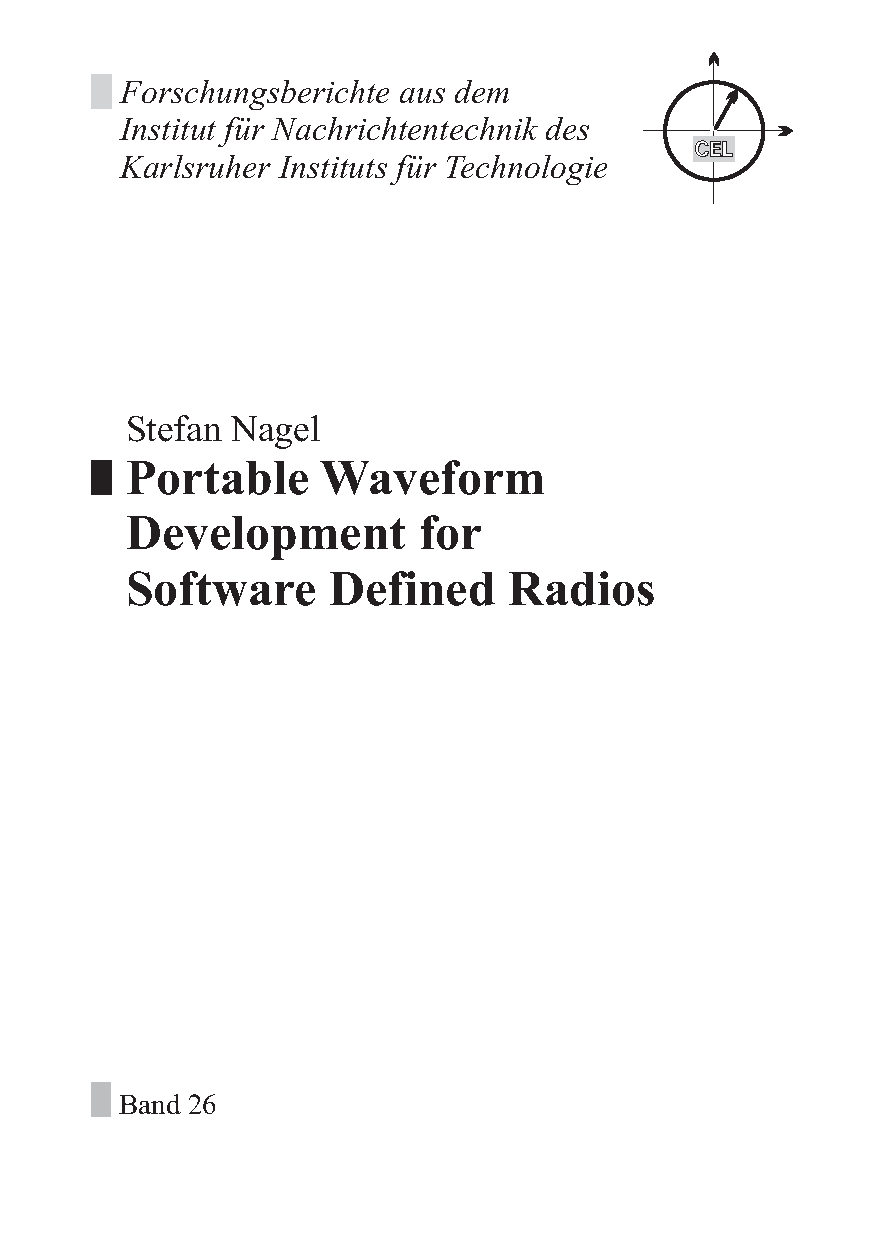
\includegraphics[]{../sonstiges/bilder/title.pdf}
%\end{figure}
%\clearpage

%%%%%%%%%%%%%%%%%%%%%%%%%%%%%%%%%%%%%%%%%%%%%%%%
% R�ckseite Schmutztitel

%%%%%%%%%%%%%%%%%%%%%%%%%%%%%%%%%%%%%%%%%%%%%%%%
%\thispagestyle{empty}
%\phantom{x}
%\vfill
%\begin{tabular}{@{}l@{ }l@{}}
%Copyright:&Institut f�r Nachrichtentechnik (CEL)\\
%&Karlsruher Institut f�r Technologie (KIT)\\
%&2011\\
%&\\
%Druck: & Frick Digitaldruck\\
%        &Br�hlstra�e 6\\
%        &86381 Krumbach\\
%&\\
%ISSN: & 1433-3821
%\end{tabular}
%\newpage

%\newcommand{\FBTableHead}{%
  \multicolumn{2}{@{}c@{}}%
  {\centering \bf Forschungsberichte aus dem Institut f�r Nachrichtentechnik}\\
  \multicolumn{2}{@{}c@{}}{\bf des Karlsruher Instituts f�r
    Technologie}\\ 
    \multicolumn{2}{@{}c}{Herausgeber: Univ.-Prof. Dr.\,rer.\,nat. Friedrich Jondral}\\
\rule{0pt}{3ex}  
  \\}
%
\begin{tabular}{@{}p{1.4cm}p{9.2cm}@{}}
  \FBTableHead%
Band 1&Marcel Kohl\\
  &{\bf Simulationsmodelle f�r die Bewertung von \newline Satelliten�bertragungsstrecken im
    \newline 20/30 GHz Bereich}\\
\rule{0pt}{3ex}%
Band 2&Christoph Delfs\\
  &\textbf{Zeit-Frequenz-Signalanalyse: Lineare und \newline quadratische
    Verfahren sowie vergleichende \newline 
    Untersuchungen zur Klassifikation von Klaviert�nen}\\%
\rule{0pt}{3ex}%
Band 3&Gunnar Wetzker\\%
  &{\bf Maximum-Likelihood Akquisition von Direct\newline Sequence Spread-Spectrum Signalen}\\
\rule{0pt}{3ex}%
Band 4&Anne Wiesler\\
  &{\bf Parametergesteuertes Software Radio \newline f�r Mobilfunksysteme}\\%
\rule{0pt}{3ex}%
Band 5&Karl L�tjen\\
  &{\bf Systeme und Verfahren f�r strukturelle \newline Musteranalysen
    mit Produktionsnetzen}\\\rule{0pt}{3ex}%
Band 6&Ralf Machauer\\
  &{\bf Multicode-Detektion im UMTS}\\\rule{0pt}{3ex}%
Band 7&Gunther M. A. Sessler\\
  &{\bf Schnell konvergierender Polynomial Expansion \newline Multiuser  Detektor mit niedriger Komplexit�t}\\
\rule{0pt}{3ex}%
Band 8&Henrik Schober\\
  &{\bf Breitbandige OFDM Funk�bertragung bei\newline hohen
    Teilnehmergeschwindigkeiten}\\\rule{0pt}{3ex}% 
Band 9&Arnd-Ragnar Rhiemeier\\
  &{\bf Modulares Software Defined Radio}\\\rule{0pt}{3ex}%
Band 10 & Mustafa Meng\"{u}\c{c} �ner\\
&{\bf Air Interface Identification for \newline Software Radio Systems}\\
\rule{0pt}{3ex}
\end{tabular}

\newpage
\begin{tabular}{@{}p{1.4cm}p{9.2cm}@{}}
 \FBTableHead
Band 11 & Fatih \c{C}apar\\
&{\bf Dynamische Spektrumverwaltung und  \newline elektronische
  Echtzeitvermarktung von \newline
Funkspektren in Hotspotnetzen}\\%
\rule{0pt}{3ex}%
Band 12 & Ihan Martoyo\\
&{\bf Frequency Domain Equalization in CDMA Detection}\\%
\rule{0pt}{3ex}%
Band 13 & Timo Wei\ss\\
&{\bf OFDM-basiertes Spectrum Pooling}\\%
\rule{0pt}{3ex}%
Band 14 & Wojciech Kuropatwi\'{n}ski-Kaiser\\
&{\bf MIMO-Demonstrator basierend \newline auf GSM-Komponenten}\\%
\rule{0pt}{3ex}%
Band 15 & Piotr Rykaczewski\\
&{\bf Quadraturempf�nger f�r Software Defined Radios: \newline Kompensation von Gleichlauffehlern}\\%
\rule{0pt}{3ex}%
Band 16 & Michael Eisenacher\\
&{\bf Optimierung von Ultra-Wideband-Signalen (UWB)}\hfill\\%
\rule{0pt}{3ex}%
Band 17 & Clemens Kl�ck\\
&{\bf Auction-based Medium Access Control}\\%
\rule{0pt}{3ex}%
Band 18 & Martin Henkel\\
&{\bf Architektur eines DRM-Empf�ngers \newline und
  Basisbandalgorithmen zur Frequenzakquisition \newline  und Kanalsch�tzung}\\%
\rule{0pt}{3ex}%
Band 19 & Stefan Edinger\\
&{\bf Mehrtr�gerverfahren mit dynamisch-adaptiver \newline Modulation
  zur unterbrechungsfreien \newline Daten�bertragung  in
  St�rf�llen}\\%
\rule{0pt}{3ex}%
Band 20 & Volker Blaschke\\
&{\bf Multiband Cognitive Radio-Systeme}\\
&\\\end{tabular}

\begin{tabular}{@{}p{1.4cm}p{9.2cm}@{}}
  \FBTableHead%
\rule{0pt}{3ex}%
Band 21 & Ulrich Berthold\\
&{\bf Dynamic Spectrum Access using OFDM-based \newline Overlay Systems}\\%
\rule{0pt}{3ex}%
Band 22 & Sinja Brandes\\
&{\bf Suppression of Mutual Interference in \newline OFDM-based Overlay  Systems}\\%
\rule{0pt}{3ex}%
Band 23 & Christian K{\"o}rner\\
&{\bf Cognitive Radio -- Kanalsegmentierung und  \newline Sch{\"a}tzung von Periodizit{\"a}ten}\\%
\rule{0pt}{3ex}%
Band 24 & Tobias Renk\\
&{\bf Cooperative Communications: Network Design and \newline Incremental Relaying}\\%
\rule{0pt}{3ex}%
Band 25 & Dennis Burgkhardt\\
&{\bf Dynamische Reallokation von spektralen Ressourcen \newline in
  einem hierarchischen Auktionssystem}\\
\rule{0pt}{3ex}%
Band 26 & Stefan Nagel\\
&{\bf Portable Waveform Development for \newline Software Defined Radios}\\
&\\\end{tabular} 

%\cleardoublepage

%\chapter*{Vorwort des Herausgebers}

%Software Defined Radios (SDRs) werden inzwischen seit zwei Jahrzehnten intensiv untersucht. Dabei stand zun�chst die Frage im Vordergrund, wie ein Funkger�t entwickelt werden kann, das mehrere verschiedene Standards unterst�tzt. Danach wurden in weitergehenden Untersuchungen Verfahren zum Software-Update, auch durch Funk�bertragung, implementiert. Dazu geh�rten auch Methoden zum Nachweis der Korrektheit der �bertragenen Software. Breitfl�chig durchgesetzt haben sich die SDR Technologien bisher im Wesentlichen in Basisstationsger�ten. Mobile Endger�te existieren vor allen Dingen als Multiband- (GSM 900, 1800, 1900) und Multistandard- (GSM, UMTS) Transceiver.

%Eine weitere wesentliche Eigenschaft, durch die sich SDRs auszeichnen k�nnen, wurde bisher zwar in der Literatur breit diskutiert, experimentell jedoch, wohl wegen der dazu notwendigen Hardware, nicht angegangen. Es handelt sich um die \textbf{Portabilit�t} von Wellenformen\footnote{Die Begriffe Standard und Wellenform werden oft als synonym angesehen. Allerdings umfassen Wellenformen, im Gegensatz zu Standards, h�ufig neben der Definition einer Luftschnittstelle auch Eigenschaften des Empf�ngers.} von einer Hardwareplattform auf eine andere. Durch das Aufkommen finanzierbarer Plattformen wie der Universal Software Radio Peripheral (USRP) von Ettus Research oder der Small Form Factor Software Defined Radio Development Platform (SFF SDR DP) von Lyrtech wird eine experimentelle Untersuchung der Portabilit�t von Wellenformen durchf�hrbar. Dabei treten Fragen nach einer Entwicklungsstrategie f�r die SDR Software unter Ber�cksichtigung der Portabilit�t sowie nach den Kosten, die eine Portierung verursacht, in den Vordergrund. Um hierf�r Antworten finden zu k�nnen, m�ssen, neben einem profunden Wissen �ber die beteiligten SDR Plattformen, Kenntnisse �ber Wellenformen bzw. Standards vorliegen. Dazu kommt die Beherrschung der notwendigen Hilfsmittel wie Programmiersprachen von MatLab �ber Python und C bis hin zu VHDL, Verilog und Assembler sowie der Umgang mit Messmitteln wie Signalgeneratoren und -analysatoren, die f�r den Nachweis erfolgreicher Arbeit, der die Interoperabilit�t zwischen auf verschiedenen Hardwareplattformen basierenden Funkger�ten umfasst, gebraucht werden.

A%uf der Basis des am KIT Institut f�r Nachrichtentechnik (Communications Engineering Lab, CEL) eingerichteten Funklabors hat Stefan Nagel die Portabilit�t verschiedener Wellenformen zwischen den beiden oben genannten Hardwareplattformen USRP und SFF SDR DP untersucht. Mit der Dissertation \emph{Portable Waveform Development for Software Defined Radios} legt er die wesentlichen Ergebnisse seiner Arbeit vor.

%Die Arbeit tr�gt insofern nachhaltig zum Fortschritt von Wissenschaft und Technik bei, als hier erstmalig, basierend auf der Model Driven Architecture (MDA) der Object Management Group (OMG), die Software f�r die Signalverarbeitung verschiedener Funk�bertragungsstandards entwickelt, implementiert und von einer Plattform auf eine andere portiert wurde. 


Karlsruhe, im 20XX\newline
Friedrich Jondral





%\cleardoublepage

\thispagestyle{empty}

\begin{center}

\vskip-3.55cm
{
%\vspace{1cm}
\huge Performance Analysis of Cognitive Radio Systems with Imperfect Channel Knowledge\\
\vskip0.25cm
}

\vfill

\vskip6.0cm

%\vskip1.0cm

%Zur Erlangung des akademischen Grades eines 
%\vfill

%\vskip0.5cm
%{\large DOKTOR-INGENIEURS}
%\vskip0.5cm
%\vfill

%von der Fakult�t f�r

%Elektrotechnik und Informationstechnik

%des Karlsruher Instituts f�r Technologie
%\vfill

%\vskip0.5cm

%genehmigte
%\vfill

%\vskip0.5cm

{\large DISSERTATION}
\vfill

\vskip0.75cm

von
\vfill

\vskip0.75cm

{\large M.Sc. Ankit Kaushik}
\vskip0.75cm



geb. in



\vskip0.15cm
\vfill


Neu Delhi, Indien

\vfill
\vskip0.75cm

\phantom{tabula}
\begin{tabular*}{11.1cm}{@{}l@{\extracolsep\fill}r@{}}
Tag der m\"undlichen Pr\"ufung:&\hfill 99 2099\\
Hauptreferent:&\hfill Prof. Dr.\,rer.\,nat. Friedrich K. Jondral\\
Korreferent:&\hfill Prof. Dr.\,-Ing. Anja Klein \\
\end{tabular*}
 \end{center}

\cleardoublepage

%
\chapter*{Abstract}
Over the last decade, wireless communication is witnessing a tremendous growth in the mobile traffic due to ever-increasing number of connected devices. Certainly, state-of-the-art standards are incapable of sustaining the substantial amount of mobile traffic, originating from these devices. It is being visualized that a major portion of this requirement can be satisfied through an additional spectrum. Due to exclusive usage, the spectrum below $\SI{6}{GHz}$ is not able to meet up the demand of additional spectrum, leading to its scarcity. To this end, Cognitive Radio (CR), along with millimeter-wave technology and visible-light communication, is envisaged as an alternative source of spectrum. The latter techniques are limited to a point-to-point communication, thus compromising mobility. In contrast, a CR system aims at an efficient utilization of the spectrum below $\SI{6}{GHz}$ -- suitable for mobile communications -- by enabling a secondary access to the licensed spectrum while guaranteeing a sufficient protection to the licensed users (also referred as a primary system). %Due to this strict constraint on the interference caused by the shared access, the performance analysis has been critical to a cognitive radio system that, in-turn, encourages its hardware deployment. 


Despite the fact that an extensive amount of literature has been dedicated to the field of CR communication, its performance analysis has been dealt inadequately from a deployment perspective. Thus, making it difficult to understand the extent of vulnerability, caused to the primary system, because of its deployment. Motivated by this fact, this thesis establishes a deployment-centric viewpoint for analyzing the performance of a CR system. Following this viewpoint, it has been identified that the interacting channels' knowledge is pivotal for the realization of cognitive techniques at the secondary transmitter. However, the aspect of channels' knowledge, particularly its effect on the performance in context to CR systems has not been clearly understood. This thesis proposes a successful integration of this knowledge -- by carrying out channel estimation -- in reference to different CR systems, namely interweave, underlay and hybrid systems. With regard to the employment of the cognitive techniques (that mainly include spectrum sensing, power control and their combination) corresponding to the aforementioned CR systems, the thesis underlines the following three aspects. 

First, this thesis establishes an analytical framework to characterize the effects such as time allocation and variation, arising due to the incorporation of imperfect channel knowledge, that are detrimental to the performance of the CR systems. In order to facilitate hardware deployment of a CR system, received power-based estimation, a novel channel estimation technique is employed for the channels existing between the primary and the secondary systems, thus fulfilling low-complexity and versatility requirements. 

Besides, this thesis follows a probabilistic approach for characterizing the variations in the system. In particular, these variation causes uncertainty in the interference at the primary system, which may disrupt the operation of the CR systems. In order to maintain the uncertainty below a desired level, new interference constraints are proposed in the thesis. Moreover, the theoretical expressions derived for the performance evaluation of the CR systems are verified by means of simulations. 


%specially for the channels between the primary and secondary systems. 
%In this context, the proposed framework captures the performance degradation, due to time allocated for performing channel estimation and the imperfect knowledge, the performance with the baseline models, constituting perfect channel knowledge. 


Second, the thesis features performance tradeoffs that determine the maximum performance of the CR systems in terms of the achievable throughput while satisfying the interference constraint. At the system design, these tradeoffs provide insights for evaluating the performance degradation in terms of throughput caused due to an inappropriate selection of the estimation and sensing durations. 

Third, using a software defined radio platform, a hardware implementation is carried out to validate the feasibility of the analysis proposed as-well-as the approach followed in the thesis. In addition, a hardware demonstrator is deployed, which in a way presents the operation of a CR system in more practical conditions. %Thereby promoting the evaluation of CR systems. 



\cleardoublepage
\chapter*{Zusammenfassung}


\cleardoublepage


%% Used to highlight text in the manuscript, will be used as dummy here
\newcommand{\tc}[1]{#1}


%% Inhaltsverzeichnis %%%%%%%%%%%%%%%%%%%%%%%%%%%%%%%%%%%%%%%
\tableofcontents %Table of contents


%% Chapters %%%%%%%%%%%%%%%%%%%%%%%%%%%%%%%%%%%%%%%%%%%%%%%%%
\mainmatter

\import{../kapitel01/}{kapitel01}
%\import{../kapitel01/}{d_kapitel01}
\cleardoublepage

\import{../kapitel03/}{kapitel03}
%\import{../kapitel03/}{d_kapitel03}
\cleardoublepage

\import{../kapitel04/}{kapitel04}
%\import{../kapitel04/}{d_kapitel04}
\cleardoublepage

\import{../kapitel05/}{kapitel05}
%\import{../kapitel05/}{d_kapitel05}
\cleardoublepage

\import{../kapitel06/}{kapitel06}
%\import{../kapitel06/}{d_kapitel06}
\cleardoublepage

\import{../kapitel07/}{kapitel07}
%\import{../kapitel07/}{d_kapitel07}
\cleardoublepage

%\begin{appendix}
%\chapter{Source Code}

\section{Source Code of the unoptimized FIR filter}
\label{sec:app_FIR}


\begin{lstlisting}[columns=flexible]
static void mdlOutputs(SimStruct *S, int_T tid)
{
  int_T             i, j;
  int_T             width;
        
  creal_T *input = (creal_T *) ssGetInputPortSignal(S, 0);
  creal_T *output = (creal_T *) ssGetOutputPortSignal(S, 0);

  width = ssGetOutputPortWidth(S,0);
       
  for (i=0; i<width; i++) {
        
    buffer[position] = input[i];
    output[i].re = 0;
    output[i].im = 0;

    for(j = 0;j<NUM_COEF;j++){
      output[i].re +=		filter_coef[j].re*buffer[(position+j)%NUM_COEF].re -filter_coef[j].im*buffer[(position+j)%NUM_COEF].im;
      output[i].im += 	filter_coef[j].re*buffer[(position+j)%NUM_COEF].im +filter_coef[j].re*buffer[(position+j)%NUM_COEF].im;
    }
    position = (position+1)%NUM_COEF;
  }   
}

\end{lstlisting}


\section{Source Code of the unoptimized FFT}
\label{sec:app_03}



\begin{lstlisting}[columns=flexible]
std::complex <float> * my_fft(int length, std::complex <float>* input)
{
  using namespace std;
  complex <float> *output   = new complex <float> [length];
  complex <float> *even_in  = new complex <float> [length/2];
  complex <float> *odd_in   = new complex <float> [length/2];
  complex <float> *even_out = new complex <float> [length/2];
  complex <float> *odd_out  = new complex <float> [length/2];
  complex <float> odd_factor;
  int i;

  if(length == 1)
    output = input;
  else
    {
    for(i = 0;i<length/2; i++){
      even_in[i] = input[2*i];
      odd_in[i]  = input[2*i+1];
      }
    even_out = my_fft(length/2,even_in);
    odd_out =  my_fft(length/2,odd_in);
		    
    for(i = 0;i<length/2; i++){
      odd_factor = polar(1.0,-2*PI*i/length) ;
      odd_factor = odd_out[i]* odd_factor;
      output[i] =          even_out[i] + odd_factor;
      output[i+length/2] = even_out[i] - odd_factor;
    }
  }
return output;
}

\end{lstlisting}


\section{Source Code of the optimized RCPC for the TCH/4.8}
\label{sec:app_01}


\begin{lstlisting}[columns=flexible]
void tch4_8_rcpc(unsigned char inVar[432], unsigned char outVar[255])
{
  unsigned char *state = malloc(292+4);
  unsigned char init[] = {0U,0U,0U,0U};
  short k,j,i;
      
  memcpy(state,init,4);
  memcpy(state + 4, inVar, 292);

  j = 0;
  i = 0;
  for (k=0; k < 146; k++){
    outVar[j+i] = (state[2*k+4] + state[2*k+3] + state[2*k])%2;
    outVar[j+i+1] = (state[2*k+4] + state[2*k+2] + state[2*k+1] + state[2*k])%2;
    if((i+2)!=65){
      outVar[j+i+2] = (state[2*k+5] + state[2*k+4] + state[2*k+1])%2;
      i+=3;
      }
    else{
      i=0;
      j+=65;
      }
    }
}
\end{lstlisting}


\pagebreak

\section{Source Code of the optimized scrambling}
\label{sec:app_02}


\begin{lstlisting}[columns=flexible]
void tch_scrambling(unsigned char inVar[432], unsigned char outVar[432])
{
  unsigned int init = 0x4183E8B7;
  unsigned int new;
  int k;
       
  for(k=0;k<432;k++){
    new = 0x80000000&(init ^ (init << 1) ^ (init << 3) ^ (init << 4) ^ (init << 6) ^ (init << 7) ^ (init << 9) ^ (init << 10) ^ (init << 11) ^ (init << 15) ^ (init << 21) ^ (init << 22) ^ (init << 25) ^ (init << 31));
    init = init >> 1 | new;
    outVar[k] = inVar[k] ^ (init >> 31);
    }   
}
\end{lstlisting}




%\end{appendix}


%%%%%%%%%%%%%%%%%%%%%%%%%%%%%%%%%%%%%%%%%%%%%%%%%%%%%%%%%%%%%
%% BIBLIOGRAPHY AND OTHER LISTS
%%%%%%%%%%%%%%%%%%%%%%%%%%%%%%%%%%%%%%%%%%%%%%%%%%%%%%%%%%%%%
%% A small distance to the other stuff in the table of contents (toc)

\backmatter

%\chapter{Acronyms}

\chapter{Acronyms and Abbreviation}
\renewcommand{\arraystretch}{1.4}
\begin{longtable}{p{0.3\columnwidth}p{0.7\columnwidth}}
%  \renewcommand{\arraystretch}{1.4}
%  \begin{tabular}{p{0.3\columnwidth}p{0.7\columnwidth}}
   	AC 	&	Average Constraint\\
   	AWGN	&	Additive White Gaussian Noise \\
	BS	&	Base Station \\
        CR 	&	Cognitive Radio \\
        CSC 	&	Cognitive Small Cell\\
	CSC-BS	&	Cognitive Small Cell-Base Station \\
	DC 	&	Direct Current \\
%% \acro{CFAR}{Constant False Alarm Rate}
  	EM	&	Estimation Model (Proposed Approach) \\
%% \acro{EM}{Expectation and Maximization}
	FDD	& 	Frequency Division Duplexing \\
	HS	& 	Hybrid System \\
%	ID	&	Indoor Device \\
%% \acro{IC}{Interference Constraint}
	IS	& 	Interweave System \\
	LSA	& 	Licensed Shared Access \\
%% \acro{MLE}{Maximum Likelihood Estimation}
%% \acro{MM}{Mixture Model}
	MC-BS	&	Macro Cell-Base Station \\
	MS	&	Mobile Station \\
	OC	&	Outage Constraint \\
	OFDM	&	Orthogonal Frequency Division Multiplexing\\
	OS	&	Overlay System \\
	PR	& 	Primary Receiver \\
	PSK	& 	Phase Shift Keying \\
	PU	& 	Primary User \\
	PT	& 	Primary Transmitter \\
	QoS/QoE & 	Quality of Service/Quality of Experience \\
%% \acro{ROC}{Receiver Operating Characteristics}
	RF	&	Radio Frequency \\
	SC 	&	Small Cell \\
	SDR 	&	Software Define Radio \\
	SMA 	&	Sub Miniature version A\\
	SNR	&	Signal to Noise Ratio \\
	SR	& 	Secondary Receiver \\
	SU	&	Secondary User \\
	ST	& 	Secondary Transmitter \\
	TDD	& 	Time Division Duplexing \\
	US	&	Underlay System \\
	USB	&	Universal Serial Bus \\
	UWB 	&	Ultra Wide Band \\
	USRP	&	Universal Serial Radio Peripheral\\
	UWB 	&	Ultra Wide Band \\

%% Abbreviations  
	cdf	&       cumulative distribution function \\
	cf.	&	confer (refer to) \\ 
 	e.g.	& 	exempli gratia (for example) \\
 	i.e.	& 	id est (that is) \\ 
 	i.i.d.	& 	independent and identically distributed \\ 
	pdf	&       probability density function \\
 	Rx	& 	Receiver \\
 	Tx	& 	Transmitter

 % \end{tabular}
\end{longtable}
  


%\begin{acronym}[ANNNNOVA]
%  \acro{AC}{Average Constraint}
%% \acro{CC}{Capacity Constraint}
%% \acro{CR}{Cognitive Relay}
% \acro{CSC}{Cognitive Small Cell}
% \acro{CSC-BS}{Cognitive Small Cell-Base Station}
%% \acro{CFAR}{Constant False Alarm Rate}
%  \acro{EM}{Estimation Model (Proposed Approach)}
%% \acro{EM}{Expectation and Maximization}
% \acro{ID}{Indoor Device}
%% \acro{IC}{Interference Constraint}
% \acro{IS}{Interweave System}
%% \acro{MLE}{Maximum Likelihood Estimation}
%% \acro{MM}{Mixture Model}
% \acro{OS}{Overlay System}
% \acro{OC}{Outage Constraint}
% \acro{PR}{Primary Receiver}
% \acro{PU}{Primary User}
% \acro{PT}{Primary Transmitter}
%% \acro{ROC}{Receiver Operating Characteristics}
% \acro{SNR}{Signal to Noise Ratio}
% \acro{SR}{Secondary Receiver}
% \acro{SU}{Secondary User}
% \acro{ST}{Secondary Transmitter}
% \acro{US}{Underlay System}
%\end{acronym}

%\section*{Abbreviations}
%\begin{table*}
%  \renewcommand{\arraystretch}{1.4}
%  \begin{tabular}{p{0.3\columnwidth}p{0.7\columnwidth}}
%   \end{tabular}



%\end{table*}
%
%\section*{Notations}
%\begin{table*}
%  \renewcommand{\arraystretch}{1.4}
%  \begin{tabular}{p{0.3\columnwidth}p{0.7\columnwidth}}
% 	$T$			& 	Frame Duration \\
% 	$\fsam$			&	Sampling Frequency \\
% 	$\tsen$			&	Sensing Time \\
% 	$\test$			&	Estimation Time \\	
% 	$\rs$			& 	Secondary Throughput at SR \\
% 	$\cz,\co$		& 	Date rate at SR without and with interference from PT  \\
% 	$\hpo$			&	Channel coefficient for the link PT-ST for IS \\
% 	$\hs$			& 	Channel coefficient for the link ST-SR for IS \\
% 	$\hpt$			& 	Channel coefficient for the link PT-SR for IS \\
% 	$\snrrcvd, \snrso$	&	Signal to noise ratio for the link PT-ST, ST-SR for IS \\
% %\acro{}[$$]{}
% 	$\snrpt$		&	Interference (from PT) to noise ratio for the link PT-SR for IS \\
% 	$\pd$			& 	Detection Probability \\ 
% 	$\pfa$		 	&	False Alarm Probability \\ 
%	$\pdd$			&	Target Detection Probability \\ 
% 	$\mu$			&	Decision Threshold \\ 
%	$\mpd$			&	Outage Constraint over Detection Probability \\ 
%	$F_{(\cdot)}$		&	Cumulative distribution function of random variable $(\cdot)$ \\
%	$f_{(\cdot)}$		&	Probability density function of random variable $(\cdot)$ \\
%	$\mathbb E_{(\cdot)}$	&	Expectation with respect to ($\cdot$) \\
%	$\p$			&	Probability measure \\
%	\textbf{T}$(\cdot)$	&	Test Statistics \\
% 	$\tilde{(\cdot)}$	&	Suitable value of the parameter ($\cdot$) that achieves maximum performance \\
% 	$\tilde{(\cdot)}$	&	Suitable value of the parameter ($\cdot$) that achieves maximum performance \\
% 	$\Ks$			& 	Number of pilot symbols used for pilot based estimation at the SR for $\hs$ \\
% 	$\Kp$			&	Number of samples used for received power based estimation at the SR for $\hpt$ \\
%   \end{tabular}
%\end{table*}
%
%



%\chapter{Notations}

\chapter{Notations and Symbols}
\renewcommand{\arraystretch}{1.4}
\begin{longtable}{p{0.3\columnwidth}p{0.7\columnwidth}}

%% System parameters
       $T$                     &       Frame duration \\
       $\fsam$                 &       Sampling frequency \\
       $\flo$                  &       Local oscillator offset frequency \\
       $\tsen$                 &       Sensing time interval \\
       $\test$                 &       Estimation time interval \\      
       $\ttesto$               &       Estimation time interval for the demonstrator \\      
       $\rs$                   &       Secondary throughput at SR \\
       $\cz,\co$               &       Date rate at SR without and with interference from PT  \\
      
%% Channel parameters 
       $\hpo$                  &       Channel coefficient for the link PT-ST for IS \\
       $\hs$                   &       Channel coefficient for the link ST-SR for IS \\
       $\hpt$                  &       Channel coefficient for the link PT-SR for IS \\
       $\snrrcvd, \snrso$      &       Signal to noise ratio for the link PT-ST, ST-SR for IS \\
 %\acro{}[$$]{}
       $\snrpt$                &       Interference (from PT) to noise ratio for the link PT-SR for IS \\

%% Probabilities and constraints
       $\pd$                   &       Detection probability \\ 
       $\pfa$                  &       False alarm probability \\ 
       $\pco$                  &       Confidence probability \\ 
       $\pdd$                  &       Target detection probability \\ 
       $\pcod$                 &       Target confidence probability \\ 
       $\mu$                   &       Decision threshold \\ 
       $\mpd$                  &       Outage constraint over detection probability \\ 
       $\ite$                  &       Interference temperature at the PR \\ 
       $\acc$	               &       Accuracy of the parameter \\	
       $\epsilon$	       &       Relative error between the normalized histogram bins and probability density function  \\	

%% Signals


%% Powers
	$\prcvd$  		&	Power received at ST over the PT-SR link (IS) PR-ST (US) \\ 
	$\prcvdpr$  		&	Power received at PR over the SR-PT link \\

	$\preg$	  		&  	Transmit power at ST, where power control mechanism is enabled	\\
	$\ptranst$ or $\pfull$ 	&  	Transmit power at ST, where power control mechanism is disabled	\\
	
%% Notations 
       $F_{(\cdot)}$            &       Cumulative distribution function of random variable $(\cdot)$ \\
       $f_{(\cdot)}$            &       Probability density function of random variable $(\cdot)$ \\
       $\mathbb E_{(\cdot)}$    &       Expectation with respect to ($\cdot$) \\
       $\p$                     &       Probability measure \\
       T$(\cdot)$  	        &       Test statistics \\
       $\tilde{(\cdot)}$        &       Suitable value of the parameter ($\cdot$) that achieves maximum performance \\
       $\tilde{(\cdot)}$        &       Suitable value of the parameter ($\cdot$) that achieves maximum performance \\
       $K$                      &       Scaling factor that holds the expected power received at the PR at interference temperature  \\
       $\Ks$                    &       Number of pilot symbols used for pilot based estimation at the SR for $\hs$ \\
       $\Kp$                    &       Number of samples used for received power based estimation at the SR for $\hpt$ \\
       $\ncchi2$                &       Non-central chi-squared distribution \\
       $\lambda_{(\cdot)}$ or $\lambda$       &       Non-centrality parameter of a non-central chi-squared distribution \\
       $a_{(\cdot)}, b_{(\cdot)}$ or $a, b$   &       Shape and scale parameters of a Gamma distribution \\

%% Special Functions
       $I_{N}(\cdot)$	        &	Modified Bessel function of first kind of order $N$ \\		
       $Q_{N}(\cdot, \cdot)$	&	Marcum Q-function \\		
\end{longtable}
  



%\section*{Abbreviations}
%\begin{table*}
%  \renewcommand{\arraystretch}{1.4}
%  \begin{tabular}{p{0.3\columnwidth}p{0.7\columnwidth}}
%	cf.	&	confer (refer to) \\ 
% 	e.g.	& 	exempli gratia (for example) \\
% 	i.e.	& 	id est (that is) \\ 
% 	Rx	& 	Receiver \\
% 	Tx	& 	Transmitter
%   \end{tabular}



\begingroup
\sloppy
\bibliographystyle{myIEEEtran}
\bibliography{IEEEabrv,../literatur/bibliography}
\endgroup


\printindex % index

\bibliographystyleK{myIEEEtran}
\bibliographyK{IEEEabrv,../literatur/mypaper}
%\bibNoteK{This thesis contains material from the following publications. Reprinted with permission.}
%\chapter*{Supervised Theses}
\addcontentsline{toc}{chapter}{Supervised Theses}

\begin{tabular*}{\textwidth}[]{p{3.5cm} p{7cm}}
	Keikavoos Afghahi & \emph{Energy Detection for Cognitive Radios}\newline(Bachelor Thesis)\\
\rule{0pt}{3ex}
Muhammad R. Raza & \emph{Deployment of Wireless Channel Model for Cognitive Relay}\newline(Master Thesis)\\
\rule{0pt}{3ex}
	Piotr Potocki & \emph{Deployment of OFDM based Cognitive Relays}\newline(Bachelor Thesis) \\
\end{tabular*}




%\chapter*{Sponsorship}
\addcontentsline{toc}{chapter}{Sponsorship}

The research visit at the Mobile and Portable Radio Research Group (MPRG) at the Virginia Polytechnic Institute and State University was supported in part by the Karlsruhe House of Young Scientists (KHYS) of the Karlsruhe Institute of Technology (KIT).
%\chapter*{Curriculum Vitae}
\addcontentsline{toc}{chapter}{Curriculum Vitae}

\section*{Personal Details}
\begin{tabular}[]{ll}
	Date of birth: & September 6th, 1980 \\
	Place of birth: & Sinsheim, Germany \\
	Citizenship: & German
\end{tabular}

\section*{Education}

\begin{tabular}[]{ll}
	
	07/2006 - 06/2011: & Research Associate, \\
										 & Karlsruhe Institute of Technology \\
	08/2009 - 10/2009: & Visiting Researcher, Virginia Tech \\
	06/2001 - 06/2006: & Dipl.-Ing., Universit�t Ulm \\
	09/1991 - 06/2000: & Anna Essinger Gymnasium, Ulm
\end{tabular}



% Used to break the theorems, proof between the columns
%\allowdisplaybreaks




\end{document}

